\scanpage{11}
$T$ torseur à droite sous \unsure{grpe|grp} $\mathbb{Z}$

\[
\deleted{\unsure{\operatorname{Aut}_{\substack{G\text{-ens}\\G\text{-}\unsure{\mathrm{var}|\mathrm{op}}}}(\unsure{D|T})
 \longrightarrow\operatorname{Aut}(G)}}
\]

\diagram{\begin{tikzcd}[ampersand replacement=\&,column sep=small]
1\arrow[r] \& \mathbb{Z}\arrow[r,"i"] \& \operatorname{Aut}(\mathbb{Z},T)\arrow[r,"p"]
 \& \operatorname{Aut}(\mathbb{Z})\arrow[r,dash]\arrow[l,dashed,bend left=28,"q_t"] \& 1
\end{tikzcd}}

$\forall t\in T$, on a
\tikz[baseline=(un.base)]{\node[inner sep=0pt] (un) {un};
\node[inner sep=0pt] at ([xshift=.35em,yshift=1.1em]un.north)
 {\unsure{\tikz{\fill (0,0) rectangle (.05,.018);}}};}
\unsure{splitting} $q_t$, défini par
% The tiny raised trace over un is retained without assigning punctuation or a function.
\[
\left\{\begin{aligned}q_t(\gamma)(t)&=t\\p(q_t(\gamma))&=\gamma\end{aligned}\right.
\]

Quelle est la relation entre $q_t$ et $q_{t'}$ ?

On \unsure{avait|aurait} $t'=t.g$, et on trouve
\[
q_{t'}=\operatorname{int}(i(g))\circ q_t
 \;:\; \gamma\longrightarrow i(g)\,q_t(\gamma)\,i(g)^{-1}
\]

[ Pour le vérifier, il suffit de voir que
% The drawn brace starts after int and ends under q_t; the equality below it is slanted.
\[
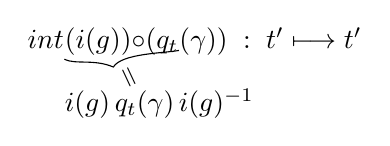
\begin{tikzpicture}[baseline=(intname.base)]
\node[anchor=base west,inner sep=0pt] (intname) at (0,0) {$\operatorname{int}$};
\node[anchor=base west,inner sep=0pt] (bracepart) at (intname.base east)
 {$(i(g))\unsure{\circ}(q_t$};
\node[anchor=base west,inner sep=0pt] at (bracepart.base east)
 {$(\gamma))\;:\;t'\longmapsto t'$};
\draw ([yshift=-.12em]bracepart.south west)
 .. controls +(.4em,-.2em) and +(-.7em,.3em) .. ([xshift=-.3em,yshift=-.4em]bracepart.south)
 .. controls +(.3em,.5em) and +(-.5em,-.1em) .. ([yshift=.2em]bracepart.south east);
\node[inner sep=0pt] at ([xshift=.2em,yshift=-.8em]bracepart.south) {\rotatebox{-65}{$=$}};
\node[anchor=base west,inner sep=0pt] at ([yshift=-2em]bracepart.south west)
 {$i(g)\,q_t(\gamma)\,i(g)^{-1}$};
\end{tikzpicture}
\]
or \quad $t'=tg$
\[
\begin{aligned}
&\deleted{q_t(\gamma)(t')=q_t(\gamma)(t)\,\gamma(g)=t.\gamma(g)}\\
&\deleted{\operatorname{int}(i(g))\,q_t(\gamma)\,(t')=}\\
&i(g)^{-1}(t')=t\qquad q_t(\gamma)\,i(g)^{-1}(t')=q_{\unsure{b|t}}(\gamma)\,t=t\\
&i(g)\,q_t(\gamma)\,i(g)^{-1}(t')=tg=t'\qquad\text{ok}\qquad ]
\end{aligned}
\]

\reversemarginpar
\margin{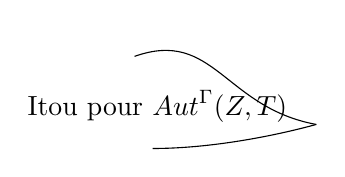
\begin{tikzpicture}[x=.65cm,y=.65cm,baseline=(itou.base)]
\node[anchor=base west,inner sep=0pt] (itou) at (0,0) {Itou pour $\operatorname{Aut}^{\Gamma}(\mathbb{Z},T)$};
% Open callout: its two left ends begin over and below Aut, not at the start of Itou.
\draw (2.1,1.15) .. controls (3.65,1.7) and (3.85,.15) .. (5.65,-.18);
\draw (2.45,-.65) .. controls (3.6,-.65) and (4.85,-.4) .. (5.65,-.18);
\end{tikzpicture}}
\normalmarginpar

\noindent\uline{Ex}\quad
\begin{tikzpicture}[baseline=(exgroup.base)]
\node[anchor=base west,inner sep=0pt] (exgroup) at (0,0) {$\mathbb{Z}=\mathbb{Z}_n$};
\node[anchor=base west,inner sep=0pt] (exsystem) at ([xshift=.7em]exgroup.base east)
 {$\left\{\begin{aligned}[b]
 \operatorname{End}\mathbb{Z}&=\mathbb{Z}_n\\
 \operatorname{Aut}\mathbb{Z}&=\mathbb{Z}_n^{*}\supset\{\pm1\}=\Gamma
 \end{aligned}\right.$};
\node[anchor=north west,inner sep=0pt] at ([xshift=.1em,yshift=-.5em]exgroup.south west)
 {$\deleted{\unsure{\Gamma\in|\Gamma\subset}}$};
\end{tikzpicture}
\margin{(\uline{NB} \unsure{si} $n=2$, $+1=-1$ dans $\mathbb{Z}_n^{*}$\ldots)}

\[
\begin{tikzpicture}[x=1cm,y=1cm,baseline=(afftop.base)]
\node[anchor=base west,inner sep=0pt] (afftop) at (0,0)
 {$\operatorname{Aff}(\mathbb{Z}_n)=\mathbb{Z}_n\mathbin{.}\mathbb{Z}_n^{*}
 \quad\text{(produit $1/2$ direct)}$};
\node[inner sep=0pt] at (.85,-.62) {\rotatebox{90}{$\subset$}};
\node[anchor=base west,inner sep=0pt] at (.25,-1.25)
 {$\operatorname{Aff}^{\{\pm1\}}(\mathbb{Z}_n)=\mathbb{Z}_n\mathbin{.}\{\pm1\}$};
% Detached angular ink mark left of the comparison; no meaning is assigned to it.
\draw[line width=.65pt] (-.66,-.39) -- (-.66,-.44) -- (-.62,-.44);
\end{tikzpicture}
\]
\margin{groupe diédral d'indice $n$, $\unsure{\mathbb{D}|D}_n$ (on suppose $n\ne2$\ldots)}

Soit $T$ torseur sous $Z$ groupe cyclique d'ordre $n\geq3$ muni d'une famille $\{u,u^{-1}\}$ de 2 gén. \deleted{d'ordre $n$.}\inserted{inverses l'un de l'}autre.
\diagram{\begin{tikzcd}[ampersand replacement=\&,column sep=small]
1\arrow[r] \& Z\arrow[r,dash,"i"] \& \operatorname{Aut}^{\pm1}(T,Z)\arrow[r,dash,"p"]
 \& \{\pm1\}\arrow[r,dash]\arrow[l,bend left=25,"q"] \& 1
\end{tikzcd}}
% archive sheet number: 10
